\section{Labeled Transition Systems}\label{sec:lts}

\begin{figure*}
\centering
\begin{boxedminipage}{.53\textwidth}
\noindent \textbf{rule} $(c.\parent == p \; \mathit{\&\&} \; c.\s[a] < x \; \mathit{\&\&} \; c.\wt[a]==$None$);$

\hspace{1cm} $\ch[c][p][\req].\enq(a,c.\s[a],x); c.\wt[a] \Leftarrow x;$

\textbf{endrule}
\end{boxedminipage}
\begin{boxedminipage}{\textwidth}
\inference[]
{\parent(c,p) & \s(c,a) < x & \wt(c,a) = \epsilon}
{\ioxe{$M_c$}
{\dt, \ch, \s, \dst, \wt, \dwt, \inp, \outp}
{\dt, \ch[ (c, p, \req) \coloneqq
(a, \s(c, a), x) \uplus \ch(c,p,\req)], \s, \dst,\\
\wt[(c,a)\coloneqq x], \dwt, \inp, \outp}}
\end{boxedminipage}
\caption{Rule in Bluespec and its corresponding LTS transliteration}
\label{both}
\end{figure*}

We make extensive use of the general theory of labeled transition
systems, a semantics approach especially relevant to communicating
concurrent systems.  As we are formalizing processors for
Turing-complete machine languages, it is challenging to prove that a
system preserves almost any aspect of processor behavior from a model
like SC.  To focus our theorems, we pick the time-honored property of
\emph{termination}.  An optimized system should terminate or diverge
iff the reference system could also terminate or diverge,
respectively.  Our basic definitions of transition systems build in
special treatment of halting, so that we need not mention it
explicitly in most contexts to come.

\begin{defn}
A \textbf{labeled transition system (LTS)} is a ternary relation, over
$\mathcal S^H \times \mathcal L^\epsilon \times \mathcal S^H$, for some sets
$\mathcal S$ of states and $\mathcal L$ of labels. We usually do not mention
these sets explicitly, as they tend to be clear from context. We write
$X^\epsilon$ for lifting of a set $X$ to have an extra ``empty'' element
$\epsilon$ (like an \texttt{option} type in ML). We write $X^H$ for lifting of
a set $X$ to have an extra ``halt'' element $H$. We also implicitly consider
each LTS to be associated with an \emph{initial} state in $\mathcal S$.
\end{defn}

For LTS $A$, we write $\io{A}{s}{s'}{\ell}$ as shorthand for $(s,
\ell, s') \in A$, and we write $A_0$ for $A$'s initial state. The
intuition is that $A$ is one process within a concurrent system. The
label $\ell$ from set $\mathcal L$ of labels is produced when $A$
participates in some IO exchange with another process; otherwise it is
an empty or ``silent'' label $\epsilon$.  As a shorthand, we sometimes
omit labels for $\epsilon$ steps.  Note that the IO exchange can be
input, output, or both, and its interpretation is dependent on the
context.


\subsection{Basic Constructions on LTSes}

From an LTS representing single-step system evolution, we often want to build
an LTS capturing arbitrary-length evolutions.

\begin{defn}
The \textbf{transitive-reflexive closure} of $A$, written $A^{*}$, is a derived
LTS.  Where $A$'s states and labels are $\mathcal S$ and $\mathcal L$, the
states of $A^{*}$ are $\mathcal S$, and the labels are $\mathcal L^{*}$, or
\emph{sequences} of labels from the original system.  $A^{*}$ steps from $s$ to
$s'$ when there exist zero or more transitions in $A$ that move from $s$ to
$s'$.  The label of this transition is the \emph{concatenation} of all labels
generated in $A$, where the empty or ``silent'' label $\epsilon$ is treated as
an identity element for concatenation.
\end{defn}

We also want to compose $n$ copies of an LTS together, with no explicit
communication between them.  We apply this construction later to lift a
single-CPU system to a multi-CPU system.

\begin{defn}
The \textbf{$n$-repetition} of $A$, written $\smulti{n}{A}$, is a derived LTS.
Where $A$'s states and labels are $\mathcal S$ and $\mathcal L$, the states of
$\smulti{n}{A}$ are $\mathcal S^n$, and the labels are $[1, n] \times \mathcal
L$, or pairs that \emph{tag} labels with which component system generated them.
These labels are generated only when the component system generates a label.
The whole system halts whenever one of the components halts.  We define the
transition relation with the following inference rules. We treat $n$-tuples as
functions keyed on numeric positions, and we write $\theta[i := v]$ for
updating $n$-tuple $\theta$ to overwrite the $i$th position with value $v$, and
we treat any label $(i, \epsilon)$ as $\epsilon$.
$$\inference[i]
{\theta(i) = a & \io{$A$}{a}{a'}{\ell} & a' \neq H}
{\io{$\smulti{n}{A}$}{\theta}{\theta[i:=a']}{i,\ell}}
\quad \inference[H]
{\io{$A$}{\theta(i)}{H}{\ell}}
{\io{$\smulti{n}{A}$}{\theta}{H}{i,\ell}}
$$
\end{defn}

Eventually, we need processes to be able to communicate with each
other, which we formalize via the $+$ composition operator. It
connects same-label transitions in the two systems, treating the label
as a cooperative communication event that may now be hidden from the
outside world, as an $\epsilon$ label.

\begin{defn}\label{plus}
Where $A$ and $B$ are two LTSes sharing labels set $\mathcal L$,
and with state sets $\mathcal S_A$ and
$\mathcal S_B$ respectively, the \textbf{communicating composition} $A + B$ is
a new LTS with states $\mathcal S_A \times \mathcal S_B$ and an empty label set,
defined as follows:
\vspace{-.2in}\begin{center}
$$\inference[$A$]
{\io{$A$}{a}{a'}{} & a' \neq H}
{\io{$A + B$}{a, b}{a', b}{}}
\quad \inference[$B$]
{\io{$B$}{b}{b'}{} & b' \neq H}
{\io{$A + B$}{a, b}{a, b'}{}}$$
$$\inference[H$_A$]
{\io{$A$}{a}{H}{}}
{\io{$A + B$}{a, b}{H}{}}
\quad \inference[H$_B$]
{\io{$B$}{b}{H}{}}
{\io{$A + B$}{a, b}{H}{}}$$
$$\inference[Join]
{\io{$A$}{a}{a'}{\ell} & \io{$B$}{b}{b'}{\ell} & a', b' \neq H}
{\io{$A + B$}{a, b}{a', b'}{}}$$
\end{center}
\end{defn}

\subsection{Refinement Between LTSes}

We need a notion of when one LTS ``implements'' another.  Intuitively,
transition labels and halting are all that the outside world
can observe. Two systems that produce identical labels and termination behavior
under all circumstances can be considered as safe substitutes for
one another. We will only need an asymmetrical notion of compatibility:

\begin{defn}\label{refines}
For some label domain $\mathcal L$, let $f : \mathcal L \to \mathcal L^\epsilon$ 
be a function that is able to replace labels with alternative
labels, or erase them altogether. Let LTSes $A$ and $B$ have the same label
set $\mathcal L$. We say that
\textbf{$A$ trace-refines $B$ w.r.t. $f$}, or $A \sqsubseteq_f B$, if:
\begin{multline*}
\forall s_A, \eta. \; \io{$A^{*}$}{A_0}{s_A}{\eta} \Rightarrow \exists s_B. \;
\io{$B^{*}$}{B_0}{s_B}{f(\eta)} \; \wedge \\
(s_A = H \Leftrightarrow s_B = H)
\end{multline*}
Each label in the trace is replaced by the mapping of $f$ on it, and
labels mapped to $\epsilon$ by $f$ are dropped. $f$ is overloaded
to denote that multi-label version when applied to $\eta$.
\end{defn}

As a shorthand, we write $A \sqsubseteq B$ for $A \sqsubseteq_\mathsf{id} B$,
for $\mathsf{id}$ an identity function, forcing traces in the two systems to
match exactly. Under this notion of identical traces, we say that $A$
is sound w.r.t. $B$.

\subsection{A Few Useful Lemmas}

The reflexivity and transitivity properties of refinement are crucial to help us
structure modular proofs.

\begin{theorem}\label{transitive}
$\sqsubseteq$ is reflexive and transitive.
\end{theorem}

Another crucial proof step is to lift a single-process result to the $n$-way
replication of that process.

\begin{theorem}\label{liftn}
If $A \sqsubseteq_f B$, then $\smulti{n}{A} \sqsubseteq_{f^n} \smulti{n}{B}$, where
$f^n$ is $f$ lifted appropriately to deal with indices ($f^n(i, \ell) =
(i, \ell')$ when $f(\ell) = \ell'$, and $f^n(i, \ell) = \epsilon$ when
$f(\ell) = \epsilon$).
\end{theorem}

We will also need a result applying to communicating compositions.

\begin{theorem}\label{liftplus}
If $A \sqsubseteq_f A'$ and $B \sqsubseteq_f B'$, then $A + B \sqsubseteq A' +
B'$. In other words, if systems $A$ and $B$ are individually simulated by $A'$ and
$B'$ on identical alteration of the traces, then the composed
system $A+B$ will be sound with respect to $A'+B'$.
\end{theorem}

%\begin{figure}
%\small
%\centering
%\begin{boxedminipage}[c]{.48\textwidth}
%%\centering
%\inference
%[Halt]
%{\theta(i) = (s, \pc) & \dec(s,\pc) = H}
%{\io{SC}{\theta,m}{H}{}}
%
%\inference
%[NonMem]
%{\theta(i) = (s, \pc) & \dec(s,\pc) = (\nm, x) \\ \exec(s, \pc, (\nm, x)) = (\pc', s')}
%{\io{SC}{\theta,m}{\theta[i \coloneqq (s', \pc')], m}{}}
%
%\inference
%[Load]
%{\theta(i) = (s,\pc) & \dec(s,\pc) = (\ld, x, a) \\ \exec(s, \pc, (\ld, x, m(a))) = (\pc', s')}
%{\io{SC}{\theta,m}{\theta[i\coloneqq(s',\pc')],m}{}}
%
%\inference
%[Store]
%{\theta(i) = (s,\pc) & \dec(s,\pc) = (\st, a, v) \\ \exec(s, \pc, (\st)) = (\pc', s')}
%{\io{SC}{\theta,m}{\theta[i\coloneqq(s',\pc')],m[a\coloneqq v]}{}}
%\end{boxedminipage}
%\caption{LTS for sequential consistency with $n$ simple processors}
%\label{Ref}
%\end{figure}
%
It is worth noting that the LTS notation described above, along with the
composition operators are very similar to the semantics of hardware designs
written in Bluespec. As an example consider an inference rule in LTS and the
corresponding code in Bluespec in Figure \ref{both}. This code was actually
written for the PowerPC system \cite{Khan:PowerPc} (we will be using this rule
later in the paper when we describe the coherent caches).

\section{Decomposing a Multi-Processor System}
\label{sec:store-atomicity}

\begin{figure}
\centering
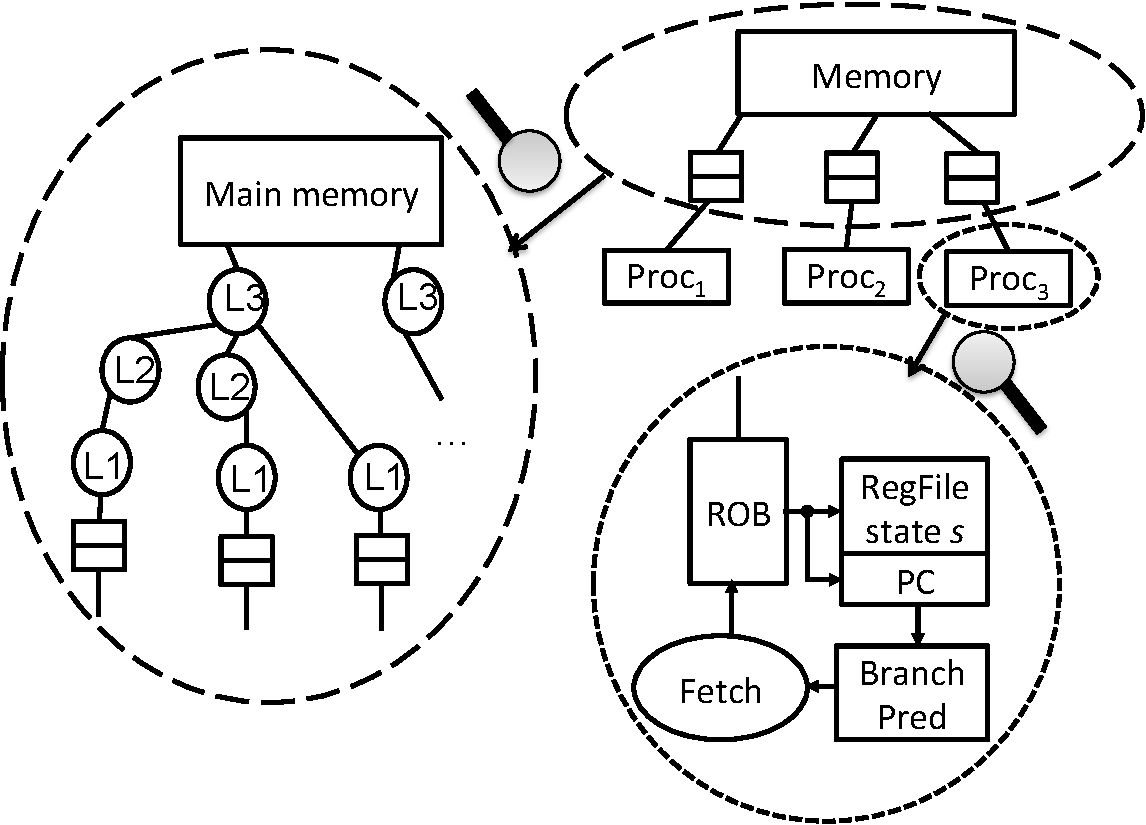
\includegraphics[scale=.43]{zoom}
\caption{Components of a multi-processors system}
\label{zoom}
\end{figure}

Most any conventional multi-processor system can be divided into 3 components as shown in
Figure \ref{zoom}. 
We show the top-level system design at top right, and we zoom in on boxes standing for the
memory system and a single processor ($P_i$).
The processor component $P_i$ can be implemented in a
variety of ways, from literal execution of instructions in program order, to complex speculation
with instructions run simultaneously to exploit parallelism. The memory component is normally implemented
using a hierarchy of caches, in order to increase the performance of the
overall system, since the latency of accessing a memory directly is very slow
compared to accessing a much smaller cache. The component between each
processor and the global memory sub-system contains local buffers, $B_i$, specific to
the processor $P_i$ they are connected to. 

\begin{figure}
\small
\centering
\begin{boxedminipage}[c]{.48\textwidth}
\inference
[Load]
{}
{\io{$M_m$}{m}{m}{p, (\ld\req,a),(\ld\resp,m(a), \_)}}

\inference
[Store]
{}
{\io{$M_m$}{m}{m[a\coloneqq v]}{p, (\st, a, v)}}

\end{boxedminipage}
\caption{LTS for a simple memory}
\label{M_m}
\end{figure}

Popular instruction set architectures do not guarantee sequential
consistency.  That is, their behavior makes it unsound to imagine that
the different processors of a shared-memory system are running
according to simple interleaving, where each instruction executes
atomically.  However, we want to emphasize that, in every weak-memory
system we are aware of, \emph{the main memory still exposes atomic
  loads and stores}!  The weaker semantics arises only because of (1)
reordering of memory instructions by the core $P_i$ and/or (2) the
properties of the local buffers $B_i$ connected to each processor
$P_i$.  For instance, if $B_i$ were a store buffer, into which the
committed stores from an in-order processor $P_i$ are enqueued, and if
any ``subsequent'' load from the same processor $P_i$ reads the latest
value from the store buffer, then one can establish that such a
multi-processor system implements the TSO~\cite{x86tsocacm10} memory
model.

So, we focus on this opportunity to simplify proof decomposition.  We
will prove that our main memory component satisfies an intuitive
\emph{store atomicity} property.  Despite the potential red herring of
the word ``atomicity,'' this specification is appropriate even for
implementation of weaker memory models than SC.  Store atomicity can
be understood via the operational semantics of Figure \ref{M_m},
describing an LTS that receives load and store requests ($\ld$ and
$\st$) from processors and sends back load responses ($\ld\resp$);
$p$ is the processor which sends and receives the request.

The memory component is composed of a \emph{hierarchy of caches}, where each
cache node (labeled like ``L1,'' ``L2,'' etc.) communicates only with its
neighbors in the graph.  Each processor has a dedicated L1 cache, from which we
do our best to satisfy all memory requests, to avoid the latency of a
round-trip with main memory.  With an L1 cache miss, we may still find a hit in
a parent cache below the level of main memory, realizing a smaller but still
significant speedup.  Therefore it is the responsibility of the hierarchy of
caches, which forms the memory sub-component, to implement the store atomicity
property. In fact, as we will prove in Section \ref{sec:cc}, the purpose of the
cache-coherence protocol is to establish this invariant for the memory
sub-component.  Concretely, we have verified a \emph{directory-based} protocol
for coordinating an arbitrary tree of caches, where each node stores a
conservative approximation of its children's states.

As an instance of the above decomposition, we will prove that a multi-processor
system with no local buffering in between the processor and the memory
components indeed implements sequential consistency. We implement a highly
speculative processor that executes instructions and issues loads out of
order, but commits instructions (once some ``verification'' is done) in order.

The processor itself can be decomposed into several components. In the zoomed-in
version of Figure \ref{zoom}, we show a highly speculative, out-of-order
issue processor. We have the normal architectural state, such as values of
registers.  Our proofs are generic over \emph{a family of instruction set
architectures}, with parameters for opcode sets and functions for executing
opcodes and decoding them from memory.  Other key components are a \emph{branch
predictor}, which guesses at the control-flow path that a processor will
follow, to facilitate speculation; and a \emph{reorder buffer (ROB)}, which
decides which instructions along that path to try executing ahead of schedule.
Our proofs apply to an arbitrary branch predictor, and they work for any
reorder buffer satisfying a simple semantic condition.

Figure~\ref{proofs} gives the overall proof structure that we employ to verify
the system of Figure~\ref{zoom}. As we will explain later, $P_\text{so}$
represents the speculative out-of-order processor, $M_c$ the cache memory,
$M_m$ the simple memory, $P_\text{ref}$ a simple decoupled processor, and
SC the simple composition of P$^n_\text{ref}+ M_m$ executing each
instruction atomically, thus implementing sequential consistency.

Our current framework establishes theorems of the form ``if system $A$ has a run
with some particular observable behavior, then system $B$ also has a run with
the same behavior.''  In this sense, we say that $A$ correctly implements $B$.
Other important properties, such as \emph{deadlock freedom} for $A$ (which
might get stuck without producing any useful behavior), we leave for future
work.

\begin{figure}
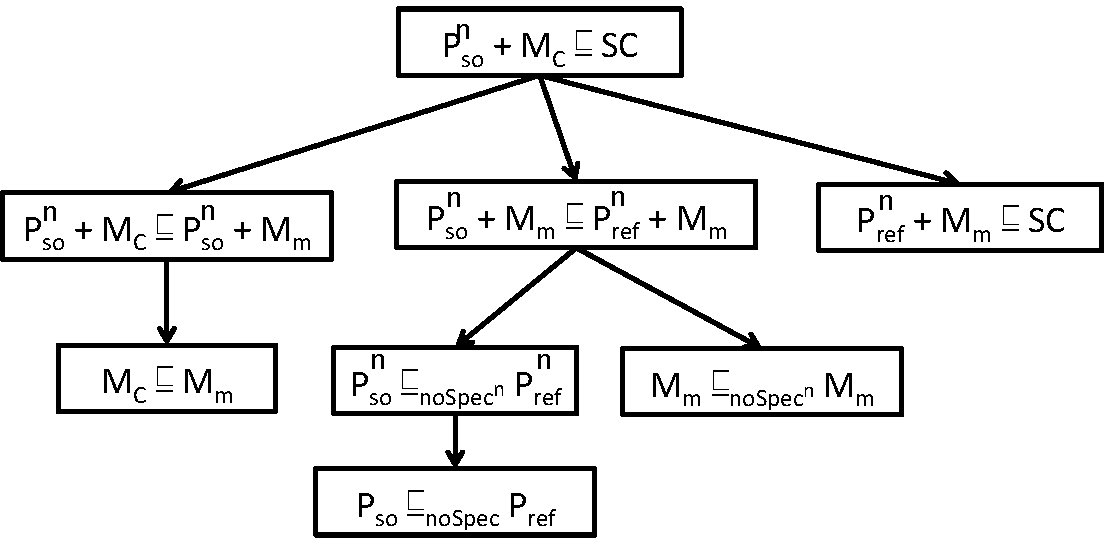
\includegraphics[scale=.45]{proofs}
\caption{Overall proof structure}
\label{proofs}
\end{figure}

